\chapter{Fundamentação Teórica}
\label{ch:fundamentacao}
\par Neste capítulo ser\~ao fundamentados os conhecimentos b\'asicos para o entendimento do trabalho.

\section{Java}

\par Java é uma linguagem de programação multiplataforma, concorrente (executa mais de uma tarefa em paralelo), baseada em classes e orientada a objetos \cite{joy2000java}.
\par A linguagem Java é compilada e interpretada. Após escrever um programa em Java, estes são salvos como código fonte com extensão ".java". Quando estes códigos fontes são compilados, um arquivo binário chamado de arquivo de classe com extensão ".class" é gerado. Estes arquivos não são executados diretamente pelos processadores, pois eles não contêm instruções para os mesmos. Os programas Java são compilados em um formato de arquivo chamado \textit{bytecode}. Desta forma, esses programas podem ser executados em qualquer sistema operacional que possua um interpretador JVM (Java \textit{Virtual Machine}) em um JRE (Java \textit{Runtime} \textit{Environment}) conforme Figura \ref{fig:ambiente java}. Assim, o código precisa ser compilado apenas uma vez para funcionar em qualquer sistema operacional que possua a configuração citada, pois os \textit{bytecodes} serão executados da mesma forma pela JVM \cite{arnold2005java}.

\begin{figure}[H]
    \centering
    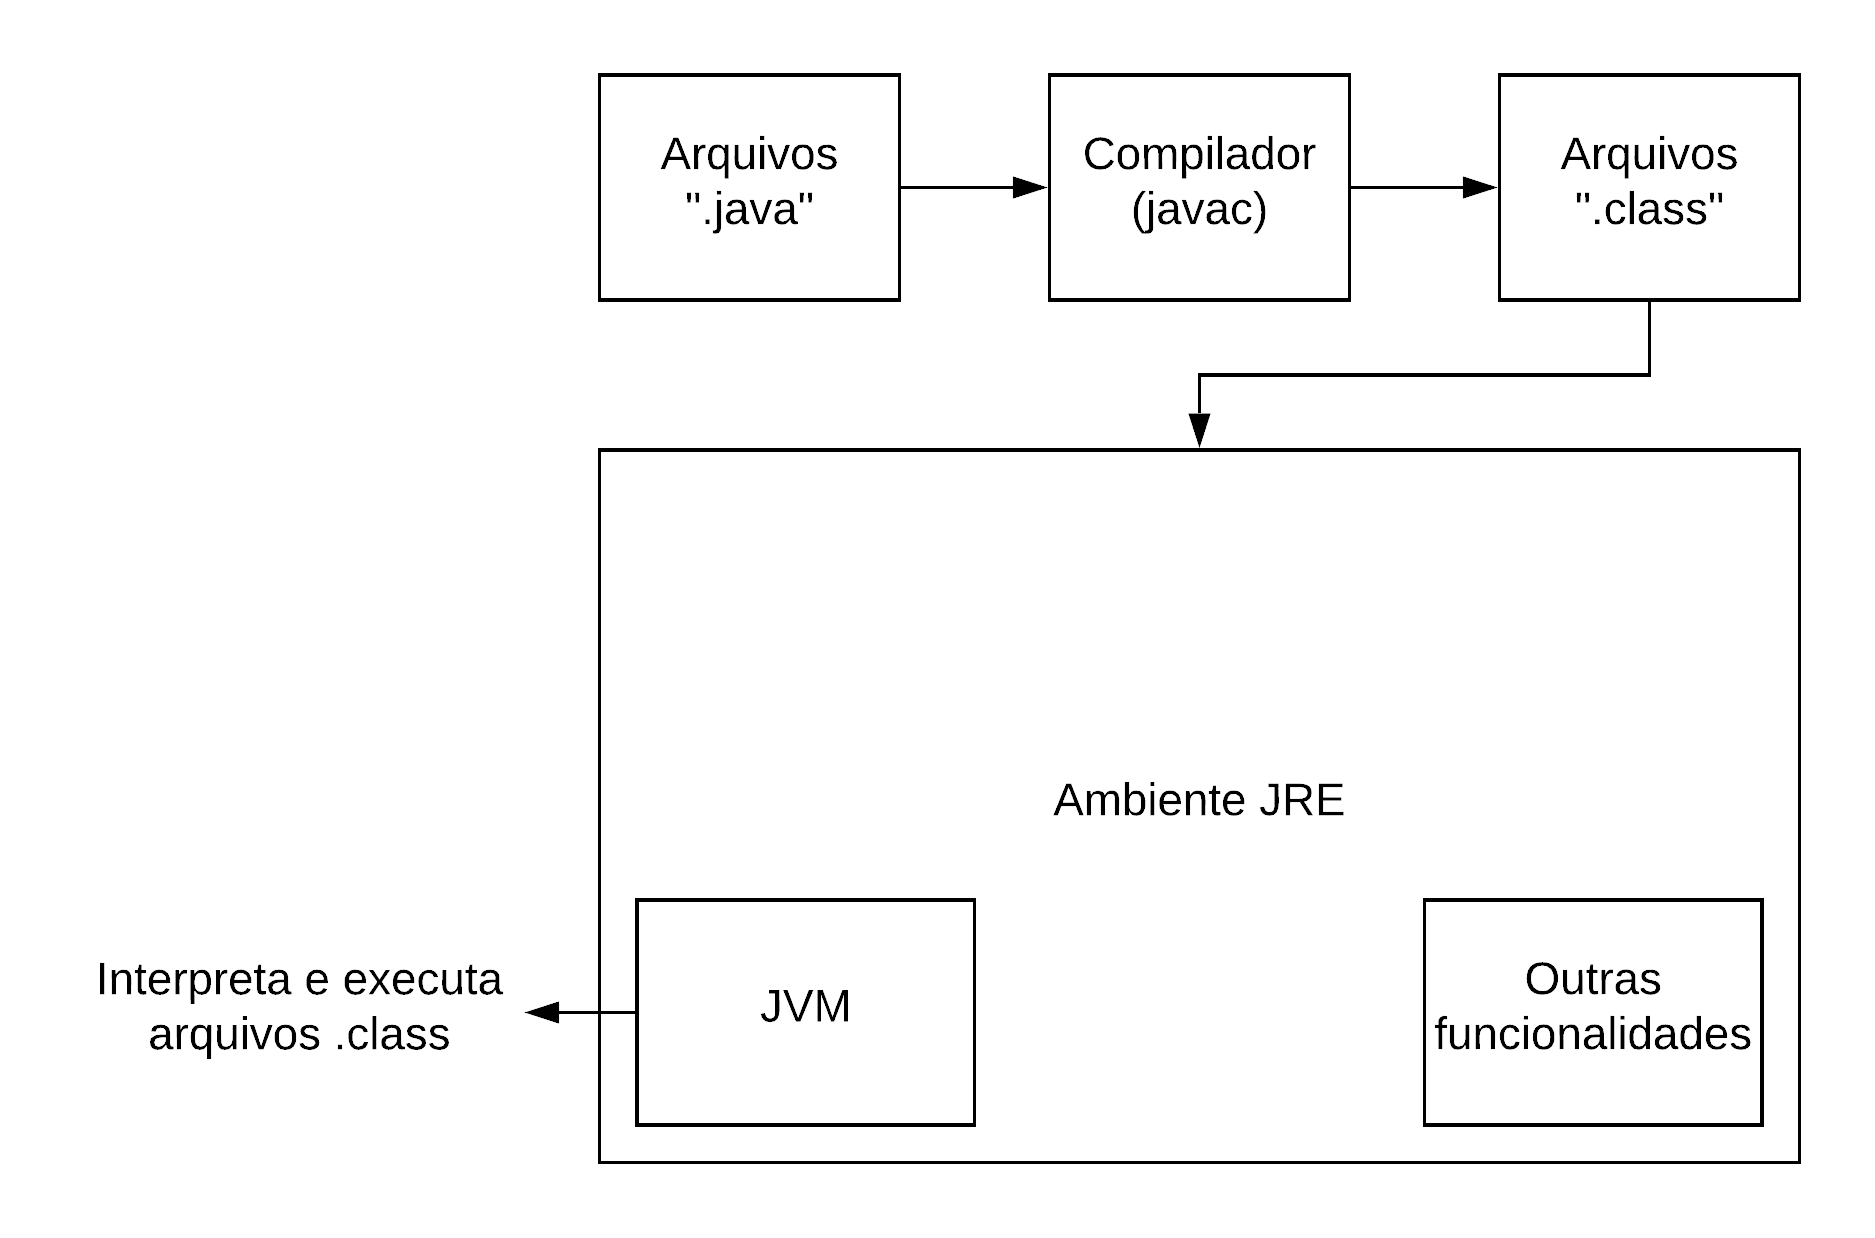
\includegraphics[scale=0.2]{src/imagens/cap1/ambiente-java.png}
    \caption{Ambiente Java}
    \label{fig:ambiente java}
    \fonte{Adaptado de \citeonline{introductionToTheJavaProgrammingEnvironment}}
\end{figure}

\par É uma linguagem fortemente tipada, isto é, as características das variáveis tem que ser definidas em tempo de compilação. Ela possui um coletor de lixo (\textit{garbage collector}) para evitar problemas de segurança como \textit{deadlock}. \cite{joy2000java}

\subsection{Reflexão}

% Magão usa \citeonline{guerra2014componentes} By: Menino
\par De acordo com \citeonline{guerra2014componentes} o conceito de reflexão pode ser definido como um processo em que um programa pode visualizar e alterar sua própria estrutura ou comportamento. As classes de reflexão disponíveis em Java localizam-se no pacote \textit{java.lang.reflect}, porém, na API (\textit{Application Programming Interface}) padrão do Java as classes deste pacote aplicam o conceito de introspecção, que é a obtenção de informações sobre sua estrutura, sem possibilidade de modificação, não existem funcionalidades de modificação disponibilizadas por padrão pela API Reflection. Com o conceito de introspecção é possível recuperar informações de acordo com o tipo atual, que são: objeto, método, anotação, interface, classe ou campo. A Figura \ref{fig:tipos-e-retornos-introspeccao} exibe os principais métodos dos tipos classe, método, objeto e atributo. 

\begin{figure}[H]
    \centering
    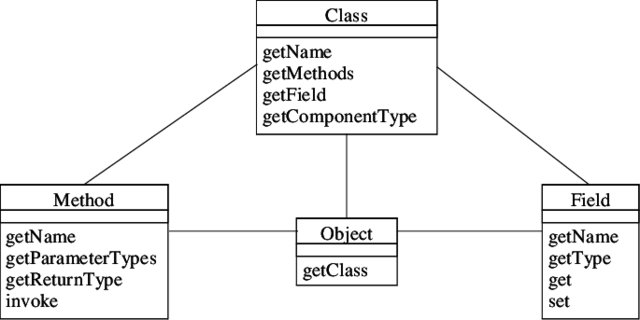
\includegraphics[scale=1]{src/imagens/cap2/metodos-introspeccao.jpg}
    \caption{Principais métodos de introspecção disponíveis por tipo}
    \label{fig:tipos-e-retornos-introspeccao}
    \fonte{\cite{parson2000using}}
\end{figure}

\par Cada tipo citado anteriormente possui sua implementação para retornar as informações necessárias, a classe \textit{Class} possui as características da classe do objeto atual em memória, e a partir dela é possível realizar as operações de introspecção vide Figura \ref{fig:introspeccao-flow}, isto é, a classe X possui uma instância de \textit{Class} com seus metadados como seu nome, construtores, assinatura dos métodos, nome e modificadores dos atributos, existência de anotações, e assim vai suscetivamente até que a classe \textit{Class} possua uma instância com suas características.

\begin{figure}[H]
    \centering
    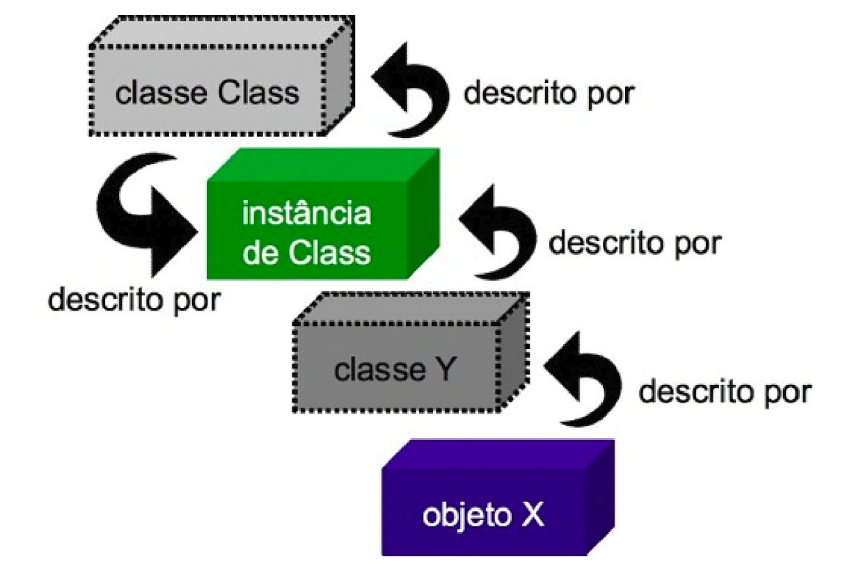
\includegraphics[scale=0.4]{src/imagens/cap2/reflection-diagrama.png}
    \caption{Fluxo de reflexão para obter informações sobre instâncias}
    \label{fig:introspeccao-flow}
    \fonte{\cite{guerra2014componentes}}
\end{figure}

\par Com reflexão é possível recuperar informações padrões sobre os dados (classes, métodos e atributos), porém não é possível realizar processos mais sofisticados como validações ou alguma regra de negócio baseando-se nisto \cite{guerra2010architectural}, para este tipo de necessidade foi criado uma forma de adição de metadados em Java, para facilitar este processo que era realizado via arquivos ou recursos não padrão, esta solução foi a criação das anotações \citeonline{jcp175metadata2002facility}.

\subsubsection{\textit{Proxy} Dinâmico}

\par Para entender o conceito de \textit{proxy} dinâmico (PD), o padrão de projeto \textit{proxy} proposto por \citeonline{gamma1995design}, exibido na Figura \ref{fig:proxy-pattern} precisa ser abordado antes. Este tem como objetivo o encapsulamento de um objeto e a implementação de sua interface, ou seja, um objeto X com uma interface Y é encapsulado por um objeto Z que implementa a interface Y também, possuindo os mesmos métodos.
%Desta forma as execuções dos métodos do objeto encapsulado são interceptadas pelo \textit{proxy}. Em outras palavras, a cada chamada de métodos do objeto encapsulado, o \textit{proxy} é executado antes conforme Figura \ref{fig:proxy-pattern}.

\begin{figure}[H]
    \centering
    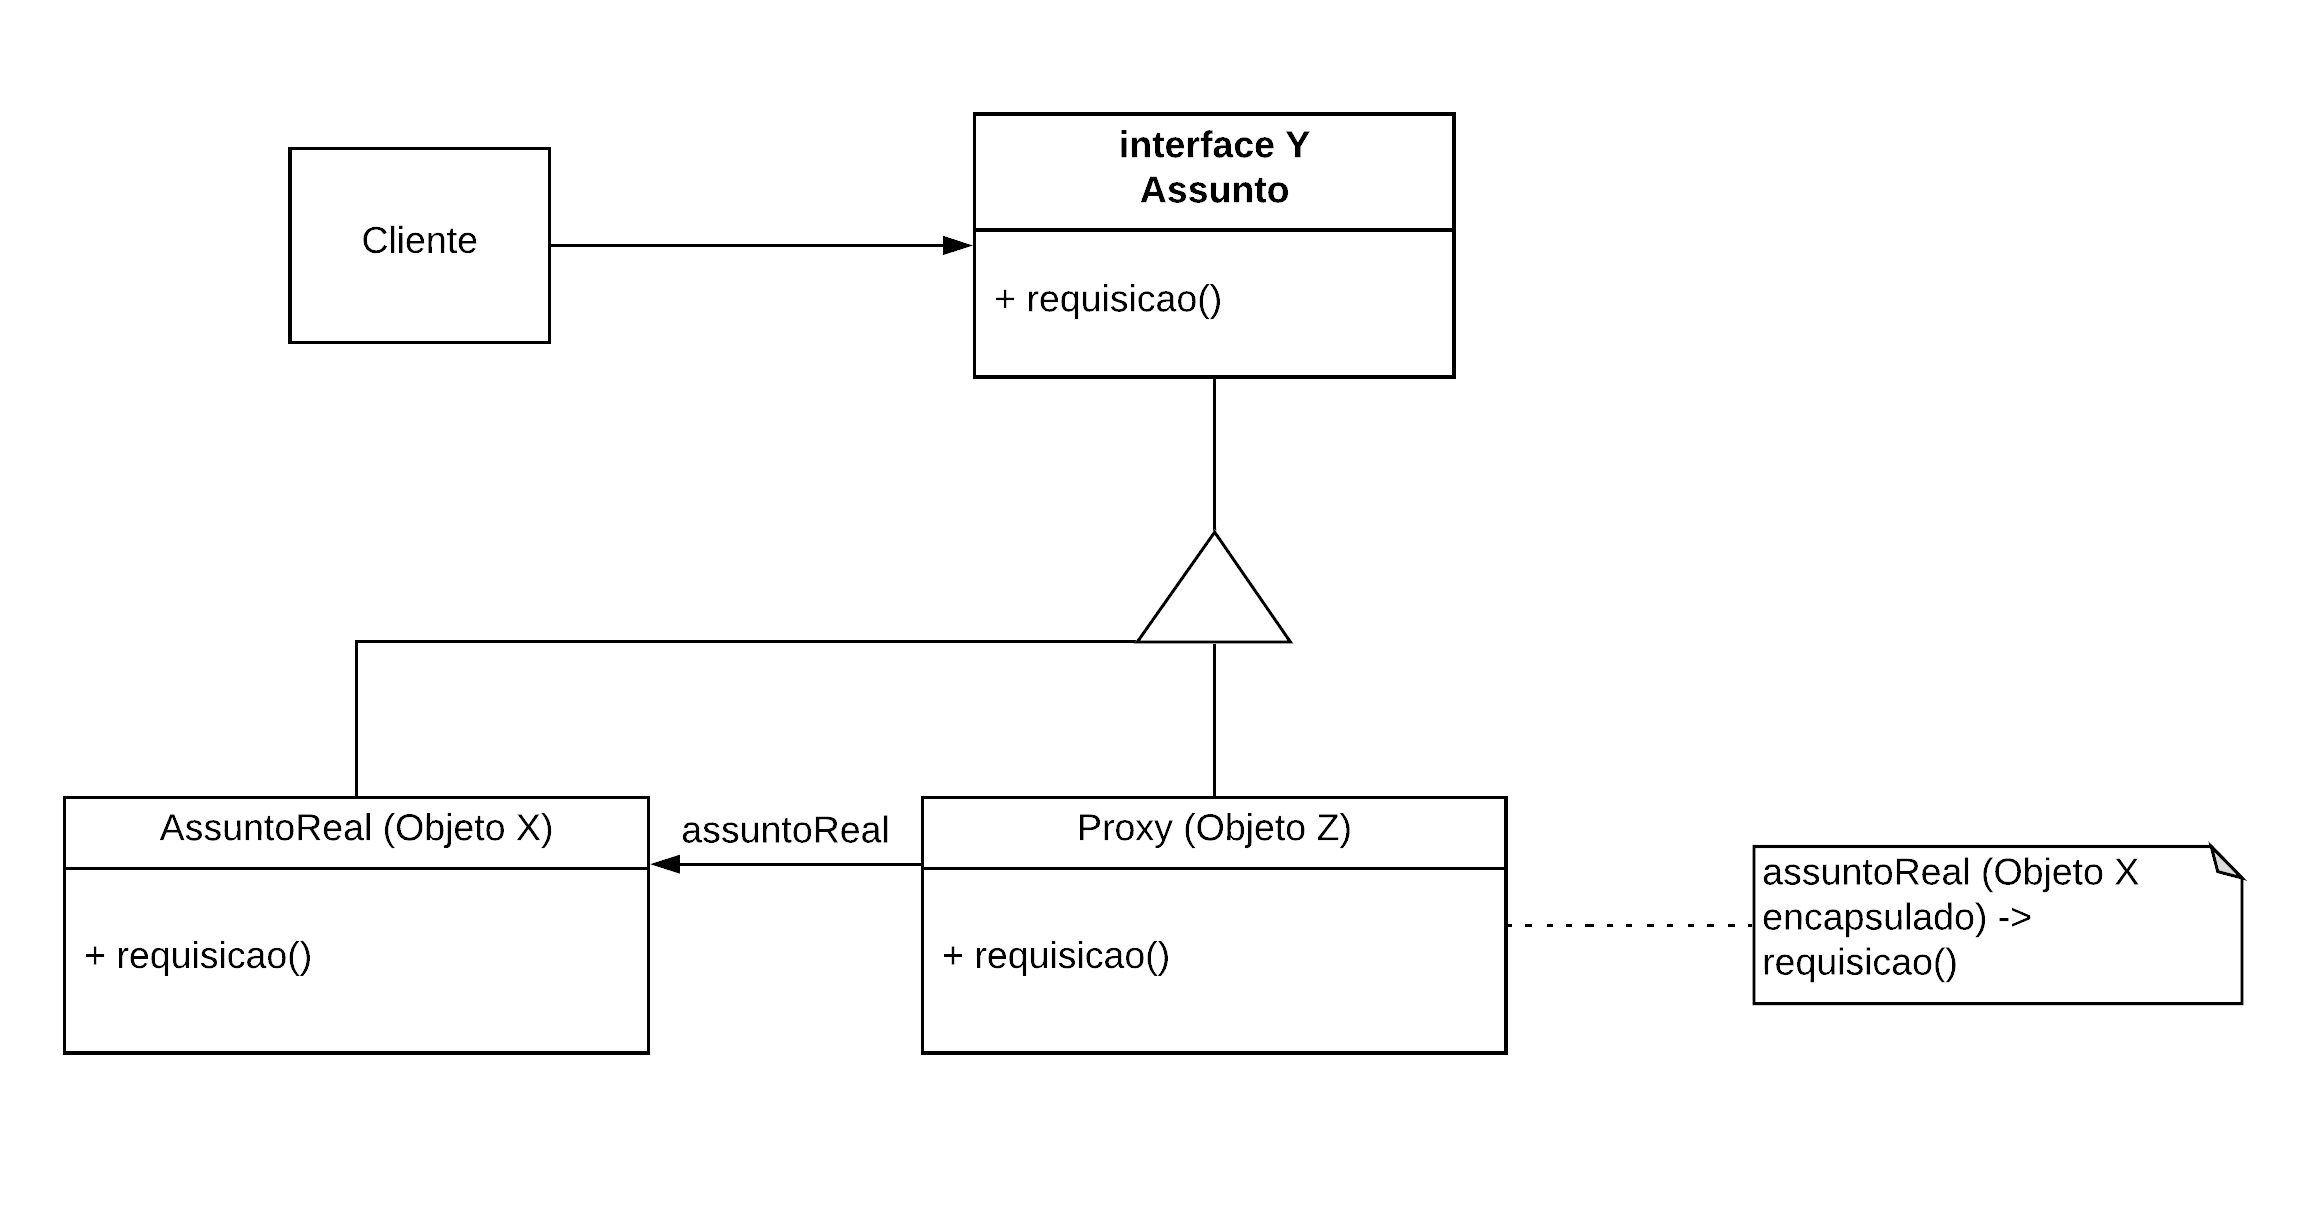
\includegraphics[scale=0.2]{src/imagens/cap2/proxy-pattern-criado.png}
    \caption{Padrão de projeto \textit{proxy}}
    \label{fig:proxy-pattern}
    \fonte{Adaptado de \cite{gamma1995design}}
\end{figure}
%, assim processos podem ser realizados de forma transparente aos dois pontos (o cliente que invocou o método e o objeto que foi invocado). 

\par Quando o cliente (Figura \ref{fig:proxy-pattern}) realiza chamadas de métodos do assuntoReal (objeto encapsulado), estas são enviadas ao \textit{proxy} primeiramente, 
portanto, todas as execuções de métodos do objeto encapsulado são interceptadas pelo \textit{proxy}. Na execução do \textit{proxy} qualquer lógica pode ser aplicada, como validações ou chamadas de outros métodos. Ao final da execução das lógicas definidas no \textit{proxy}, a responsabilidade é devolvida ao objeto encapsulado. Um problema na utilização de \textit{proxies} é a dependência da interface, pois caso outro objeto precise ser encapsulado sua interface também precisa ser implementada, ou seja, outro \textit{proxy} deverá ser criado.
PD, é um recurso disponibilizado pela API reflexão (\textit{reflection}) do Java, a fim de interceptar invocações de objetos como apresentado na \ref{fig:proxy-dinamico} 

\subsection{Anotação}

\par Anotações em Java, são utilizadas para definição de metadados, isto é, informações sobre algo, estas podem ser inseridas em: Pacotes; Classes; Interfaces; Métodos; Atributos; Parâmetros; Construtores; e em Anotações \citeonline{jcp2005annotation269}. O local onde uma anotação pode ser inserida é definido pela anotação \textit{@Target} que recebe de um a N parâmetros do Enum tipo \textit{java.lang.annotation.ElementType}\footnote{É interessante restringir o local onde as anotações podem ser inseridas para evitar uma má interpretação durante sua recuperação via reflexão}, a Tabela \ref{tab:targets} exibe os parâmetros disponíveis e seu escopo. Quando uma anotação é inserida fora de seu escopo um erro de compilação com a mensagem \textit{"The annotation @NomeDaAnotação is disallowed for this location"} \citeonline{joy2000java}.

\begin{table}[H]
    \centering
    \begin{tabular}{|l|l|}
        \hline
        Parâmetro & Escopo \\ \hline
        TYPE & Classes, Enums, Anotações, Interfaces e  Pacotes \\ \hline
        FIELD & Atributos \\ \hline
        METHOD & Métodos \\ \hline
        PARAMETER & Parâmetros \\ \hline
        CONSTRUCTOR & Construtores \\ \hline
        LOCAL\_VARIABLE & Variáveis locais (dentro de métodos) \\ \hline ANNOTATION\_TYPE & Anotações \\ \hline
        PACKAGE & Pacotes \\ \hline
        TYPE\_PARAMETER  & Tipos genéricos definidos em Métodos, Classes e Interfaces \\ \hline
        TYPE\_USE & Variáveis com tipos genéricos \\ \hline
\end{tabular}
    \caption{Parâmetros e restrições de anotações}
    \label{tab:targets}
    \fonte{Adaptado de Java specification}
\end{table}

Definido o escopo de atuação da anotação é preciso definir seu escopo de duração, isto é, até onde ela será mantida no código, pois as anotações não são persistidas até o tempo de execução sem uma anotação chamada \textit{@Retention}. Esta define o ciclo de vida da anotação, na Tabela \ref{tab:retentions} seus parâmetros, que são de um a N Enum do tipo \textit{java.lang.annotation.RetentionPolicy} são explicados \citeonline{joy2000java}.

\begin{table}[H]
    \centering
    \begin{tabular}{|l|l|} \hline
        Parâmetro & Ciclo de vida\\ \hline
        SOURCE    & Anotações não são carregadas nos arquivos ".class"\\ \hline
        CLASS     & Anotações são mantidas nos arquivos ".class" mas não são carregados pela JVM\\ \hline
        RUNTIME   & Anotações são mantidas pelos arquivos ".class" e carregados pela JVM \\ \hline
    \end{tabular}
    \caption{Parâmtros da anotação retention e seu tempo de duração}
    \label{tab:retentions}
    \fonte{Adaptado de Java specification}
\end{table}

\par O parâmetro \textit{SOURCE} é utilizado geralmente por IDE's (\textit{Integrated Development Environment}), para adicionar algum comportamento específico como a anotação \textit{@SuppressWarnings} que serve para ignorar algum aviso, presente em IDE's como o Eclipse e o IntelliJ IDEA. Para que uma anotação seja recuperada em tempo de execução é preciso adicionar a \textit{RetentionPolicy Runtime}, devido ao comportamento padrão da anotação \textit{@Retention} que é o valor \textit{CLASS} \cite{joy2000java}.

\par É possível adicionar propriedades em uma anotação para complementar comportamentos ou informações que esta proporcionará, as propriedades permitidas são: Tipos primitivos; Enums; Class (Apenas a classe Class); String; Anotações; e Arrays dos tipos anteriores conforme Figura \ref{fig:propriedades-anotacoes}.

\begin{figure}[H]
    \centering
    \begin{java}
Anotacao anotacoes();
Class classes();
String strings();
boolean boleanos();
byte bytes();
char chars();
double doubles();
float floats();
int inteiros();
long longs();	
short shorts();
Anotacao[] arrayDeAnotacoes();
Class[] arrayDeClasses();
String[] arrayDeStrings();
boolean[] arrayDeBoleanos();
byte[] arrayDeBytes();
char[] arrayDeChars();
double[] arrayDeDoubles();
float[] arrayDeFloats();
int[] arrayDeInteiros();
long[] arrayDeLongs();	
short[] arrayDeShorts();
    \end{java}
    \caption{Propriedades permitidas em anotações}
    \label{fig:propriedades-anotacoes}
    \fonte{Adaptado de \cite{joy2000java}}
\end{figure}

\par Na Figura \ref{fig:declaracao-anotacao} uma anotação é declarada para exemplificação, esta é mantida até o tempo de execução e pode ser adicionada em outras anotações e métodos. Por padrão, nenhum comportamento é adicionado ou alterado com a adição de uma anotação, isto é feito a partir de métodos que verificam sua existência, como reflexão citada no capítulo anterior \cite{bloch2004jsr}. 

\begin{figure}[H]
    \centering
    \begin{java}
@Target({ ANNOTATION_TYPE, METHOD })
@Retention(RUNTIME)
public @interface Anotacao {
}
    \end{java}
    \caption{Declaração de uma anotação}
    \label{fig:declaracao-anotacao}
    \fonte{Produção do autor}
\end{figure}

\textit{Frameworks} baseados em reflexão e metadados são \textit{softwares} que utilizam a reflexão para obtenção de metadados, estes disponibilizam anotações com o valor \textit{Runtime} para sejam lidos posteriormente \cite{guerra2009pattern}.

\section{\textit{Framework}}

\par Um \textit{framework} é considerado um \textit{software} incompleto que é especializado com o comportamento de uma aplicação externa \cite{johnson1988designing}. Este determina a arquitetura que a aplicação utilizará, sua organização, como: convenções de nomes, arquitetura do projeto, arquivos externos de configuração e/ou anotações. Isto é definido para que o desenvolvedor tenha que se preocupar apenas com o problema que está resolvendo. A forma que o \textit{framework} realiza esta organização deve ser baseada no que é mais viável para solucionar a situação comum em relação ao problema encontrado, permitindo que a tarefa repetitiva ou específica seja reaproveitada em novos projetos.
Baseado nisso \textit{frameworks} permitem que aplicações com estruturas semelhantes sejam criadas, facilitando a manutenção, padronização e legibilidade do código, entretanto, isto restringe o desenvolvedor a solução que o \textit{framework} aplica, não permitindo que determinados caminhos sejam seguidos ou certas decisões sejam tomadas no projeto \cite{gamma2009padroes}. A ideia por trás dessa restrição citada é a inversão de controle existente, onde os \textit{frameworks} chamam o código que foi desenvolvido, não o contrário, desta forma muitas vezes é realizada a injeção de dependências neste código criado, que é o fornecimento de implementações de interfaces em tempo de execução, a Figura \ref{fig:inversao-controle} exemplifica uma situação em que existe a inversão de controle em um ambiente Web, onde a requisição é recebida pelo servidor e a responsabilidade inicial é do framework, este realiza o processamento inicial passando a requisição por filtros e outras validações e depois passa a responsabilidade para as classes criadas pelo desenvolvedor final. Existem pontos extensíveis em frameworks, estes são chamados de \textit{hotspots} e servem para especializações como no exemplo anterior (Figura \ref{fig:inversao-controle}) em que os blocos roxos são os hotspots fornecidos, estes são implementados pelos desenvolvedores pois é possível atender requisitos como filtros genéricos que precisam ser verificados e restrições recuperadas de metadados, porém a tratativa específica não tem como ser atendida em todos os caos e precisa ser implementada via hotspots, geralmente frameworks disponibilizam algumas especializações prontas, mas caso seja necessário outras podem ser criadas para situações em que as soluções existentes não resolverem o problema, por outro lado, ao contrário dos hotspots existem os frozenspots (blocos azuis da Figura \ref{fig:inversao-controle}) que são trechos que não devem ser alterados ou especializados de formas diferentes, são as funcionalidades e processos automatizados pelo framework \cite{markiewicz2001object}

\begin{figure}[H]
    \centering
    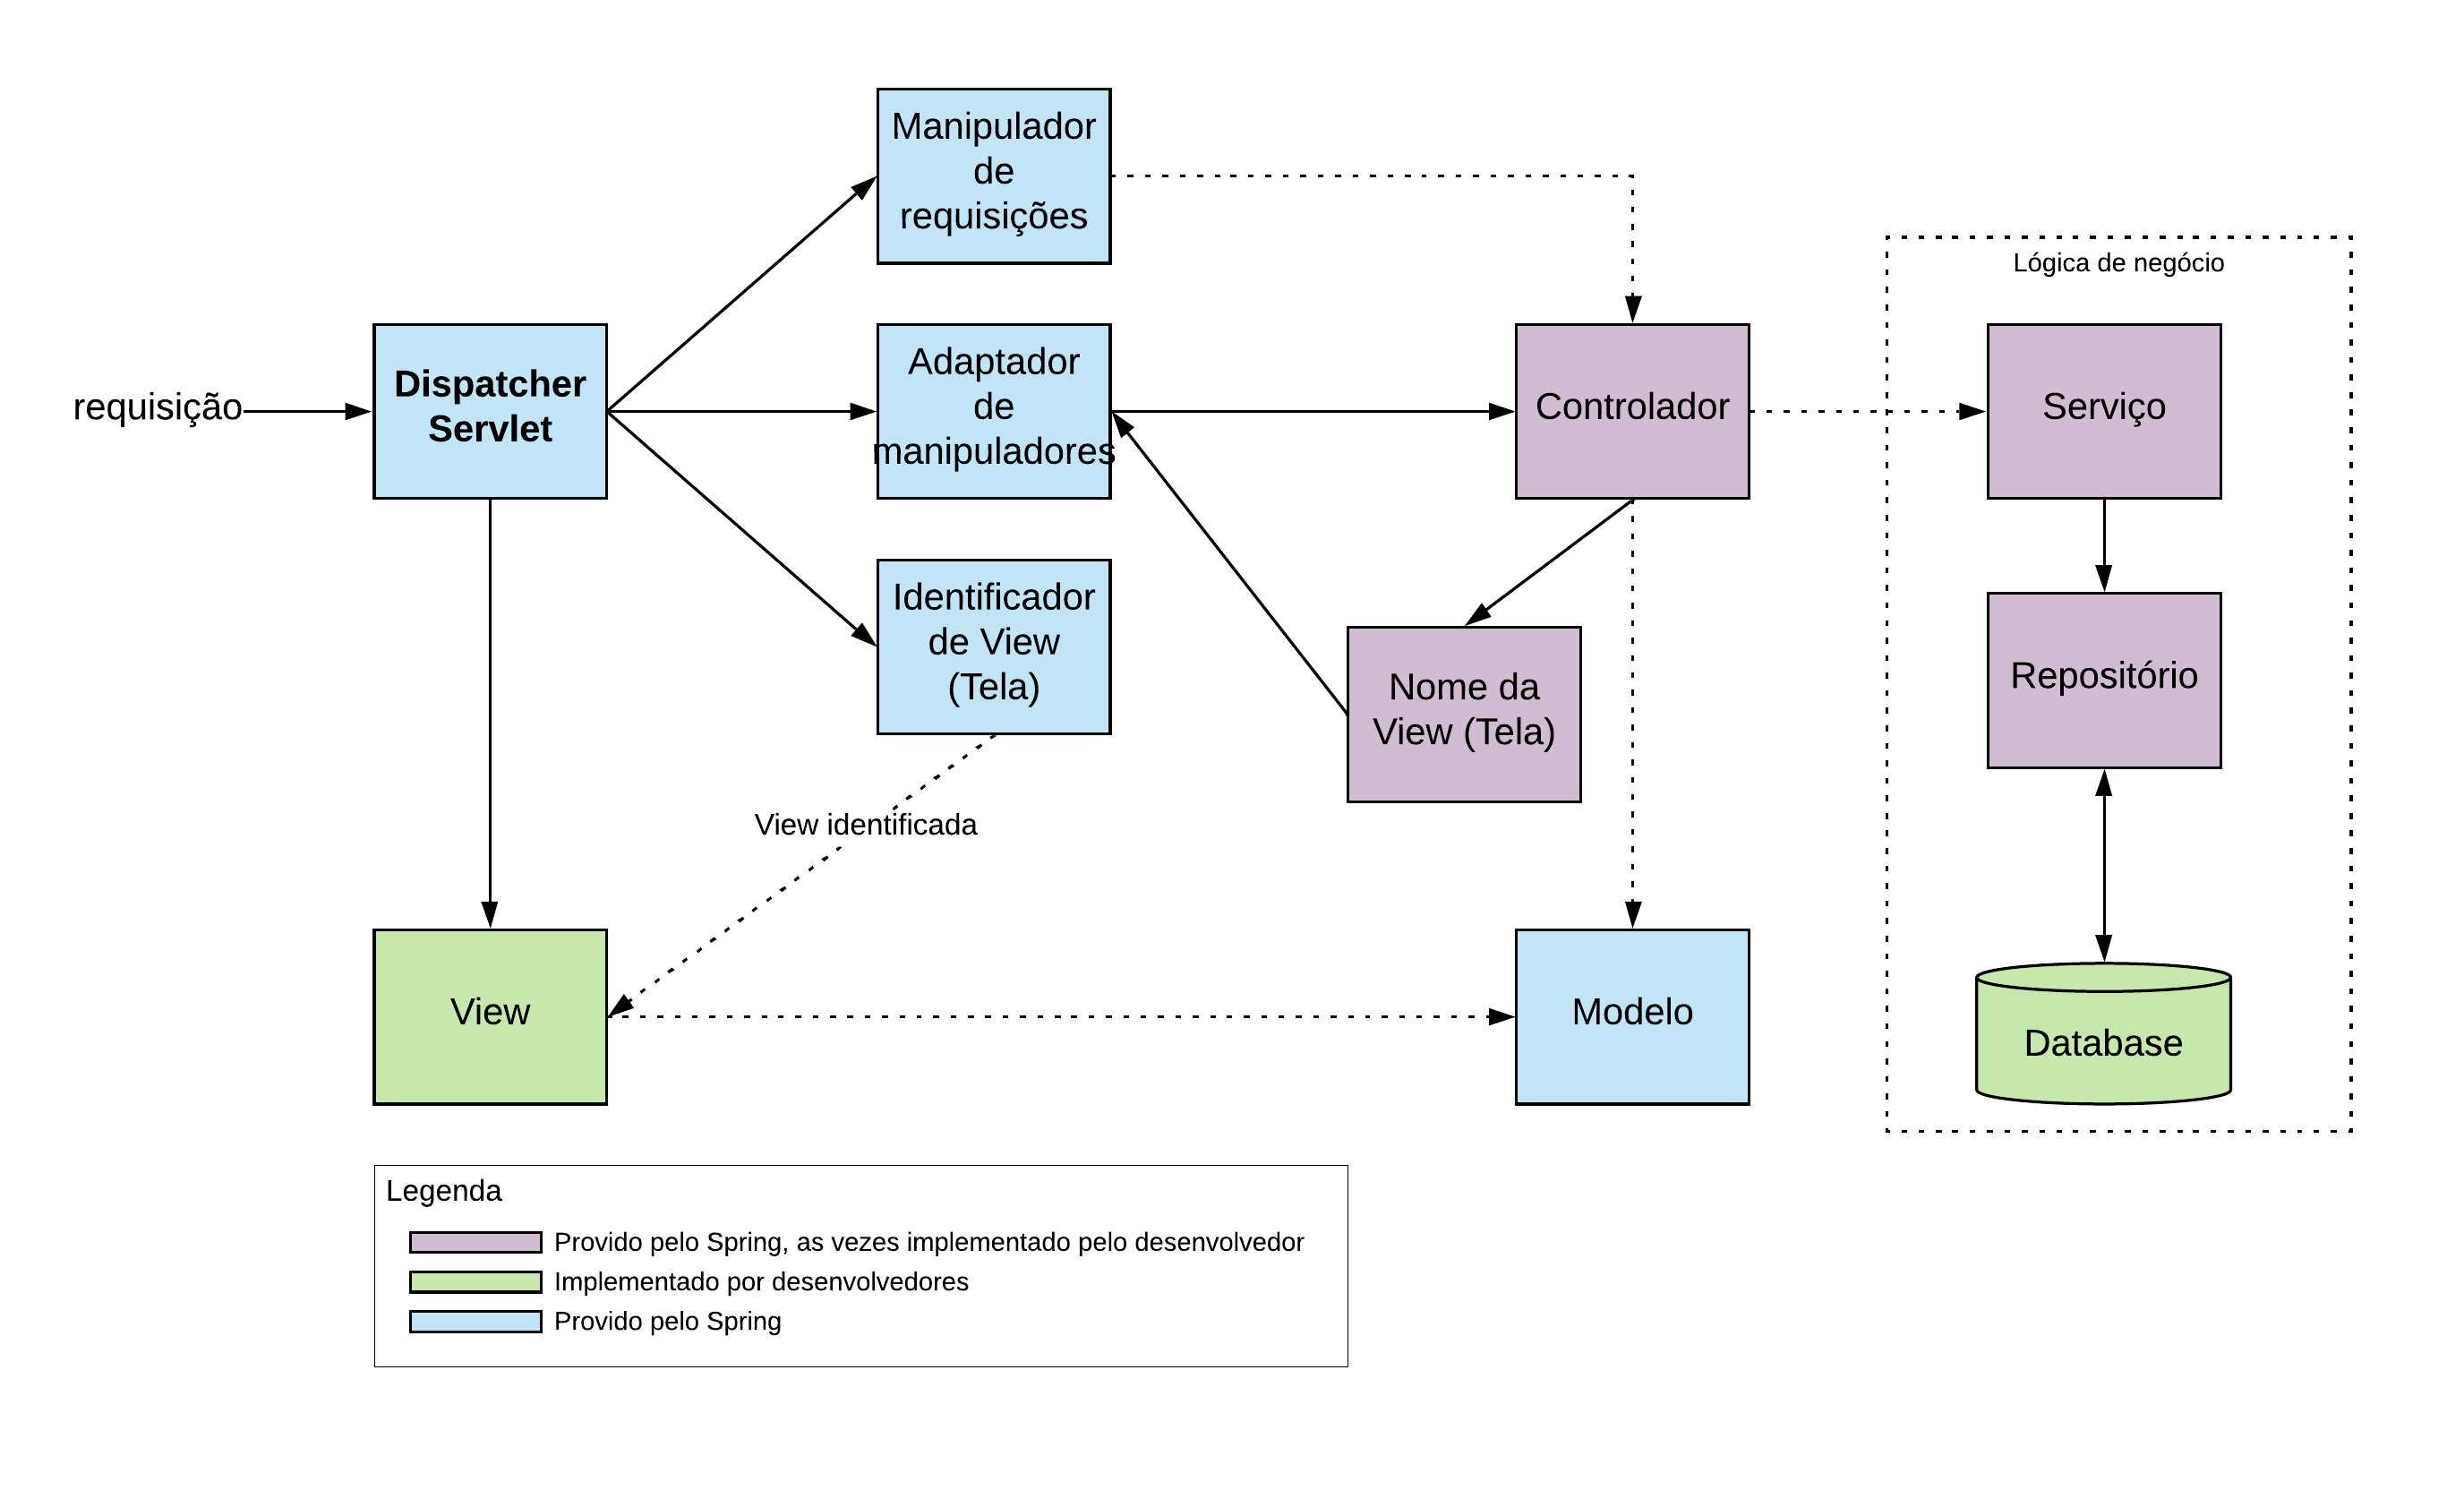
\includegraphics[scale=0.2]{src/imagens/cap2/arquitetura-spring-traduzida.png}
    \caption{Inversão de controle}
    \label{fig:inversao-controle}
    \fonte{Origem \cite{spring-mvc-architecture}}
\end{figure}

\subsection{Frameworks baseados em Reflexão e Metadados}

\par Frameworks baseados em metadados revolucionaram a ideia do desenvolvimento destas soluções, devido ao problema da limitação de expressão que existia. Era possível adicionar comportamentos no framework via implementações de interfaces, heranças de classes abstratas (hook methods), convenções de nome e arquivos externos de configuração. Convenções de nome como getters e setters dos Java Beans por exemplo, são formas de adição de metadado que podem ser utilizados por frameworks quando estes possuem algum valor semântico, a Figura \ref{fig:spring-qyery-method} exibe como query methods são utilizados pelo Spring JPA, nele os parâmetros de consulta são inseridos no nome do método e o SQL é criado em tempo de execução, o Spring identifica que a interface possui query methods com a extensão de interfaces parametrizadas em sua documentação, estas são: Repository, CrudRepository, JpaRepository. Convenções de nome são limitadas e quando é necessário alguma definição mais complexa não é possível criar o metadado com esta abordagem. 

\begin{figure}
    \centering
    \begin{java}
public interface CrudRepository<T, Integer> {
    Optional<T> findById(Integer id);
}
    \end{java}
    \caption{Query method Spring JPA}
    \label{fig:spring-qyery-method}
    \fonte{\citeonline{gierke_darimont_strobl_paluch_bryant_2019}}
\end{figure}

Arquivos externos são muito verbosos pois precisam descrever precisamente onde as modificações acontecerão ou onde estão agregando informações, a Figura \ref{fig:arquivo-metadado} exibe um arquivo de configuração básica de persistência de uma entidade para o Hibernate.

\begin{figure}[H]
    \centering
    \begin{xml}
<?xml version="1.0"?>
<!DOCTYPE hibernate-mapping PUBLIC "-//Hibernate/Hibernate Mapping DTD 3.0//EN"
"http://hibernate.sourceforge.net/hibernate-mapping-3.0.dtd">

<hibernate-mapping>
    <class name="br.fatec.sjc.exemplo.Pessoa" table="pessoa" catalog="exemplo">
        <id name="pessoaId" type="java.lang.Integer">
            <column name="PES_ID" />
            <generator class="identity" />
        </id>
        <property name="nome" type="string">
            <column name="PES_NOME" length="50" not-null="true" unique="false" />
        </property>
        <property name="cpf" type="string">
            <column name="PES_CPF" length="11" not-null="true" unique="true" />
        </property>
    </class>
</hibernate-mapping>
    \end{xml}
    \caption{Configuração de persistência de uma classe via XML}
    \label{fig:arquivo-metadado}
    \fonte{Adaptado de \cite{xml-hibernate-configuration}}
\end{figure}

\par Para resolver estes problemas as anotações foram criadas conforme JCP 269 \citeonline{jcp2005annotation269}. Com as anotações os metadados são inseridos no próprio código, deixando a semântica mais fluídas e menos verbosas, na Figura \ref{fig:classe-metadado} é realizada a mesma configuração da Figura \ref{fig:arquivo-metadado}, neste exemplo é possível analisar a facilidade que as anotações trouxeram para o desenvolvimento, possibilitando que metadados sejam adicionados de uma forma mais natural, fazendo parte da própria linguagem.

\begin{figure}
    \centering
    \begin{java}
@Entity
@Table(name = "pessoa", uniqueConstraints = { @UniqueConstraint(columnNames = { "cpf" }) 
})
public class Pessoa implements Serializable {

	@Id
	private Integer id;
	@Column(nullable = false)
	private String nome;
	@Column(nullable = false)
	private String cpf;

    // Getters e setters omitidos

}
    \end{java}
    \caption{Configuração de persistência de um classe via anotação}
    \label{fig:classe-metadado}
    \fonte{Adaptado de \citeonline{annotation-configuration-hibernate}}
\end{figure}

O uso de anotações é chamado de programação orientada a atributos \cite{buschmann2007pattern}, com a adição desta nova funcionalidade adição de metadados complexos é possível, a leitura destes também é facilitada pois as anotações fazem partes da API, assim os problemas citados nesta seção foram solucionados.

\section{Gamificação}

\par Gamificação pode ser definido como a utilização de conceitos de design de jogos, como: Ganho de pontos, \textit{ranking}, troféus, e \textit{rewards} em aplicações de outros contextos \cite{deterding2011gamification}. \textit{Softwares} de e-commerce, sites de e-learning, são alguns exemplos de contextos onde a gamificação pode ser aplicada. Um exemplo de aplicação que utiliza gamificação é a Foldit \cite{burke2012behind}, que utiliza conceitos de pontos e troféus em um jogo de quebra cabeça, para na verdade, prever a estrutura da proteína humana \cite{deterding2011gamification}. O propósito da gamificação é fazer com que a utilização das aplicações não diminua com o tempo e proporcione experiências melhores ao usuário, pois as conquistas adquiridas durante a utilização incentivam a continuidade. A Psicologia Comportamental trata desta abordagem utilizada na gamificação como reforços positivos e negativos \cite{skinner1990behavior}. Os reforços positivos tem como objetivo estimular indivíduos a repetirem ações a partir da agregação de algo, na gamificação isto é aplicado com a ideia da aquisição das conquistas, e como já dito, isto estimula o indivíduo a continuar os processos que está fazendo para receber mais conquistas. Por outro lado, existem os reforços negativos, que incentivam o indivíduo a realizar o processo inverso do que foi feito para receber este estimulo, isto é, o comportamento é condicionado a partir de processos para evitar alguma situação, como por exemplo perder pontos ou perder posições no ranking se tratando de gamificação, isto gera efeitos colaterais como fuga e esquiva no indivíduo e este aprende naturalmente a evitar reforços negativos \cite{linehan2015gamification}. Nas duas formas é possível condicionar o indivíduo a realizar atividades para chegar a um propósito.

\section{Esfinge Project}

\par Esfinge Project\footnote{O projeto está disponível no endereço: http://esfinge.sf.net.} é um projeto \textit{open-source} iniciado em 2011 por Dr. Eduardo Guerra junto a GSW, que tem como objetivo a criação de soluções reutilizáveis para um desenvolvimento ágil, um produto final flexível e de fácil manutenção.
\par O projeto disponibiliza 9 frameworks até o momento, estes são: QueryBuilder, Comparison, Guardian, AOM Role Mapper, SystemGlue, Gamification, Metadata, Classmock, ReTest.
\par Todos os frameworks citados acima seguem uma filosofia que consiste em: Configuração de metadados para que o comportamento desejado ocorra; Componentes que podem ser integrados a aplicações de forma simples; Pontos de extensão para criação de novas funcionalidades; Remover a preocupação com a solução que o framework disponibiliza, permitindo que o desenvolvedor foque apenas em sua aplicação específica \cite{esfinge2011}.

\subsection{Esfinge Gamification}

\par O Esfinge Gamification\footnote{A documentação do projeto está disponível no endereço: http://esfinge.sourceforge.net/Gamification.html.} é um \textit{framework} que aplica lógica gamificação para \textit{softwares} que necessitam destes processos. Independente do domínio do \textit{software} é possível utilizar o \textit{framework}, pois este é desacoplado de lógicas da aplicação, sua responsabilidade é a tratativa dos dados de gamificação, portanto, pode ser integrado a qualquer programa Java, permitindo que o desenvolvedor foque na solução que está trabalhando, e deixe as responsabilidades de gamificação para o \textit{framework}  \cite{esfinge2011}.

%conforme Figura \ref{fig:esfinge-gamification-plugado}
%\begin{figure}[H]
%    \centering
%    \caption{Diagrama de %atuação do Esfinge %Gamification}
%    \label{fig:esfinge-ga%mification-plugado}
%\end{figure}

\par O comportamento do framework é especificado via metadados conforme a filosofia dos projetos Esfinge, estes são anotações que podem ser adicionadas em softwares, a Tabela \ref{tab:anotacoes-gamification} detalha as opções disponíveis. Existem quatro tipos de processos implementados pelo \textit{framework}, estes são: Ponto, Ranking, \textit{Reward}, Troféu vide Figura \ref{fig:arquitetura-esfinge-gamification}.

\begin{table}[H]
\resizebox{\textwidth}{!}{
\begin{tabular}{|l|l|}
\hline
Anotação & Comportamento \\ \hline
\begin{tabular}[c]{@{}l@{}}@PointsToUser, @RankingsToUser, \\ @RewardsToUser, @TrophiesToUses\end{tabular} & Incremento de conquista para o usuário atual. \\ \hline
\begin{tabular}[c]{@{}l@{}}@RemoveRankings, @RemovePoints, \\ @RemoveReward, @RemoveTrophy\end{tabular} & Eliminação de conquista do usuário atual. \\ \hline
\begin{tabular}[c]{@{}l@{}}@PointToParam, @RankingToParam,\\ @RewardToParam, @TrophyToParam\end{tabular} & \begin{tabular}[c]{@{}l@{}}Incremento de conquistas para outro usuário, \\ ou seja, a ação do usuário logado no sistema \\ gera pontos para outro usuário.\end{tabular} \\ \hline
@RemovePointsToParam & \begin{tabular}[c]{@{}l@{}}Remove Pontos de outro usuário seguindo a \\ lógica de atribuição, isto é, o usuário que está\\ logado no sistema desencadeia este comportamento.\end{tabular} \\ \hline
@TrophyWhenReachPointLimit & \begin{tabular}[c]{@{}l@{}}Cria um EventListener para adicionar\\ troféus quando uma quantidade de \\ Pontos for alcançada.\end{tabular} \\ \hline
\end{tabular}
}
\caption{Anotações disponibilizadas pelo Esfinge Gamification}
    \label{tab:anotacoes-gamification}
    \fonte{Adaptado de \cite{esfingegamification2011}}
\end{table}

\begin{figure}[H]
    \centering
    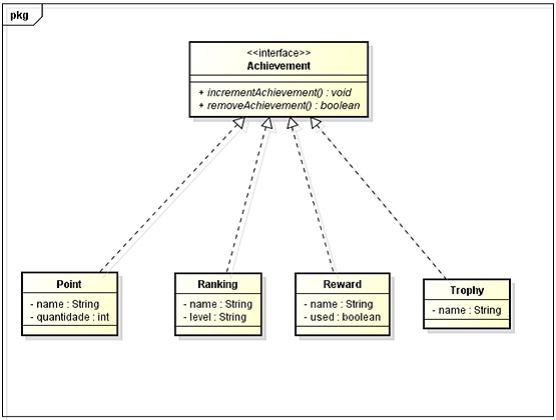
\includegraphics{src/imagens/cap2/estrutura-conquistas.png}
    \caption{Conquistas implementadas no projeto Esfinge Gamification}
    \label{fig:arquitetura-esfinge-gamification}
\end{figure}

\subsubsection{Características das conquistas disponibilizadas}

\par Ponto: Tem como intenção atribuir determinada quantidade de pontos e seu tipo, por exemplo, uma conquista que atribui 10 pontos de moedas de ouro, onde moedas de ouro são o tipo e 10 os pontos atribuídos. 
\par Ranking: Se assemelha a uma hierarquia militar, onde o ranking é de status, não de posições. Por exemplo, um usuário possui o status iniciante quando começa a utilizar a aplicação, e quando realiza algum processo específico, é premiado com o status de intermediário ou avançado.

\par Troféu: Pode ser atribuído uma vez apenas, por exemplo, caso um usuário realize um processo e receba um troféu por isto, na próxima vez que realizar o mesmo processo não receberá outro troféu.

\par \textit{Reward}: É uma conquista que é consumida, ou seja fica indisponível após ser usada. Por exemplo, um \textit{reward} de bônus de ligações será recebido não consumido por padrão, só será consumido quando uma ligação for realizada com seu recurso de bônus.

\subsection{Pontos de extensão}

O \textit{framework} possui dois pontos de extensão (\textit{hotspots}), onde novos comportamentos podem ser adicionados, quando necessário. Desta forma é possível aplicar outras lógicas de gamificação, implementando a interface \textit{Achievement} (Figura \ref{fig:arquitetura-esfinge-gamification}) disponível no pacote \textit{net.sf.esfinge.gamification.achievement}, caso os comportamentos disponibilizados pelo \textit{framework} não sejam adequados \`a determinada situação. Também é possível adicionar novos comportamentos estendendo a classe abstrata \textit{Game}, disponível no pacote \textit{net.sf.esfinge.gamification.mechanics}, que possui a lógica de gerenciamento dos dados de gamificação e consequentemente o controle das conquistas, isto é, a adição, atualização, consulta e remoção destas. Além de sua forma de armazenamento, que possui implementações para: Arquivo de propriedades; Banco de dados relacional; Banco de dados não relacional; e em memória \cite{esfinge2011}.


\subsection{Esfinge Guardian}

\par Autorização em software pode ser resumida na pergunta: "Este assunto pode acessar este recurso?". Onde assunto pode ser definido como um usuário ou sistema externo com a intenção de realizar um processo em um ambiente controlado, e recurso como algo que está sob proteção, algo não publico \cite{bartsch2011authorization}.
\par O Esfinge Guardian é um \textit{framework} para a aplicação de autorizações em \textit{softwares}, seguindo a filosofia do Esfinge Project citado anteriormente. Este aplica os seguintes modelos de controle de acesso:

\begin{itemize}
    \item ABAC: Attribute Based Access Control é um controle de acesso lógico que verifica atributos de objetos, em um determinado ambiente e assunto, para validar se o objeto poderá ou não realizar o acesso naquela situação baseado nas politicas definidas \cite{hu2015attribute}
    \item MAC: Mandatory access control é um controle de acesso que é definido por apenas uma entidade no sistema, e apenas esta entidade pode realizar a alteração das permissões definidas, geralmente este tipo de controle de acesso é utilizado para informações sensíveis, é semelhante a um sistema militar \cite{lindqvist2006mandatory}.
    \item RBAC: \textit{Role-based access control} é uma forma de controle de acessos baseado em funções, isto é, cada objeto (este podendo ser um usuário ou um ativo), possui uma ou mais funções que o permitem realizar determinados processos de acordo com seu nível hierárquico, semelhante a uma empresa \cite{sandhu2000nist}.
    
\noindent\subsubsection{Pontos de extensão}
\end{itemize}